\documentclass[letterpaper, 12pt]{article}

\usepackage[utf8]{inputenc}
\usepackage[english, spanish]{babel}
\usepackage{fullpage}
\usepackage{graphicx}
\usepackage{amsmath}
\usepackage{enumitem}
\usepackage{chngcntr}
\usepackage{setspace}
\usepackage{url}
\usepackage{csquotes}
\usepackage{float}
\usepackage{verbatim}
\usepackage{tabularx}
\usepackage{amsmath}
\usepackage{caption}
\usepackage{bm}
\usepackage{wrapfig}
% \usepackage{hyperref}

\counterwithin{figure}{section}
\renewcommand{\thesection}{\arabic{section}}
\renewcommand{\thesubsection}{\thesection.\arabic{subsection}}
\renewcommand{\baselinestretch}{1.5}

\usepackage[style=numeric, maxnames=6, minnames=3, backend=biber, parentracker=true, sorting=none]{biblatex}
\DefineBibliographyStrings{english}{%chktex-file 1 chktex-file 6
      andothers = {\em et\addabbrvspace al\adddot}
}

\addbibresource{./Bibliography/bibliography.bib}

\usepackage{array}
\usepackage{enumitem}

\setlength{\parskip}{0pt}

\newcommand{\bolditalic}[1]{\textbf{\textit{#1}}}

\newcommand{\Celsius}[0]{°$\mathcal{C}$}
\newcommand{\Kelvin}[0]{°$\mathcal{K}$}
\newcommand{\Fahrenheit}[0]{°$\mathcal{F}$}

% chktex-file 44

\begin{document}

\begin{titlepage}
      \centering
      
\includegraphics[width=0.3\textwidth]{Images/logo_utb.png}\par\vspace{1cm}
      {\scshape\LARGE Universidad Tecnológica de Bolívar \par}
      \vspace{1cm}

      {\scshape\Large FÍSICA CALOR Y ONDAS \par}
      \vspace{.2cm}

      % chktex-file 8
      {\scshape\Large Grupo 1 \par}
      \vspace{2cm}
      % chktex-file 8
      \slshape {\Large \bfseries{}LAB 8 - EFECTO COMPTON\\}
      \slshape {\large Verificación de la pérdida de
            energía de los fotones dispersados \\}
      \slshape {\small \bfseries{} Guía de laboratorio No. 8}
      \vspace{4cm}

      \slshape {\itshape{} Mauro González, T00067622 \\}
      % \slshape {\itshape{} German De Armas Castaño, T00068765 \\}
      % \slshape {\itshape{} Angel Vega Rodriguez, T00068186 \\}
      % \slshape {\itshape{} Juan Jose Osorio Ariza, T00067316 \\}
      % \slshape {\itshape{} Jorge Alberto Rueda Salgado, T00068722 \\}
      \vfill
      Revisado Por \\
      Duban Andres Paternina Verona\\
      {\large \today\par}
\end{titlepage}

% ! ----------------------------------------------------------------------|>
\section{Introducción}

El efecto Compton, un fenómeno fundamental en la física de
partículas que demuestra la naturaleza corpuscular de los
fotones.

El efecto Compton, observado por el físico estadounidense
A.H. Compton en 1923, consiste en la dispersión de rayos X
por parte de electrones en reposo, lo que resulta en un
cambio en la longitud de onda de los fotones dispersados.
Esta observación llevó a la conclusión de que la radiación
electromagnética también exhibe propiedades corpusculares.

% ! ----------------------------------------------------------------------|>
\section{Objetivos}

\subsection{Objetivo general}

Verificar experimentalmente el efecto Compton mediante la
dispersión de radiación gamma por un material dispersante.
Esto implica cuantificar el cambio en la longitud de onda y
energía de los fotones dispersados y comprobar si estos
resultados se ajustan a la teoría de Compton.

\subsection{Objetivos específicos}

\begin{itemize}[label=$\triangleright$]
      \item Calcular la energía promedio de los fotones gamma para
            diferentes ángulos de dispersión y determinar a qué rango
            del espectro electromagnético corresponden.

      \item Evaluar experimentalmente si la ecuación de Compton es
            válida comparando los valores calculados con las mediciones
            experimentales y sus incertidumbres.

      \item Calcular la longitud de onda de Compton para el electrón
            utilizando los datos experimentales y compararla con el
            valor aceptado.
\end{itemize}

% ! ----------------------------------------------------------------------|>
\section{Preparación de la practica}

% + --------------------------------------------------------------|>
\subsection{\cite{radiacion_rayos_x}~\cite{radiacion_rayos_gamma}}

Los fotones que integran el haz de rayos X emitido por el
tubo presentan una distribución continua en energías con
valores comprendidos, teóricamente, entre 0 y un valor
máximo que corresponde al valor de tensión o kilovoltaje
aplicado al tubo de rayos X. En efecto, si aplicamos una
tensión, por ejemplo, de 90 kV entre el cátodo y el ánodo,
los electrones adquirirán una energía de 90 keV, y al
chocar contra el ánodo, perderán energía emitiendo
radiación de frenado. Los fotones de rayos X emitidos
tendrán energías comprendidas entre 0 y 90 keV. Esta
distribución de energías forma un espectro continuo.

\begin{figure}[H]
      \begin{center}
            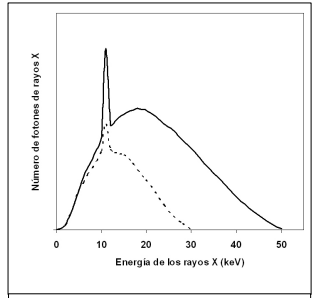
\includegraphics[width=.7\linewidth]{Images/Image_1.png}
            \caption{}
      \end{center}
\end{figure}

Los rayos gamma son la luz más poderosa y energética que
existe. Su rango de energía es tan grande que no tienen
bien definido un límite superior de energía. No hay nada en
nuestro planeta capaz de producir los rayos gamma de más
alta energía, por lo que necesitamos observar el Universo
en busca de las fuentes cósmicas más violentas y exóticas
para detectarlos y estudiarlos. Los rayos gamma son, por
tanto, la luz más energética posible. El Cherenkov
Telescope Array (CTA) observará un rango energético de
rayos gamma sin precedentes, desde los 20
Gigaelectronvoltios* (GeV) hasta los 300
Teraelectronvoltios (TeV) - billones a trillones de veces
más energética que la luz visible.

% + --------------------------------------------------------------|>
\subsection{\cite{Moebs_2021}}

\begin{wrapfigure}{l}{.4\textwidth}
      \begin{center}
            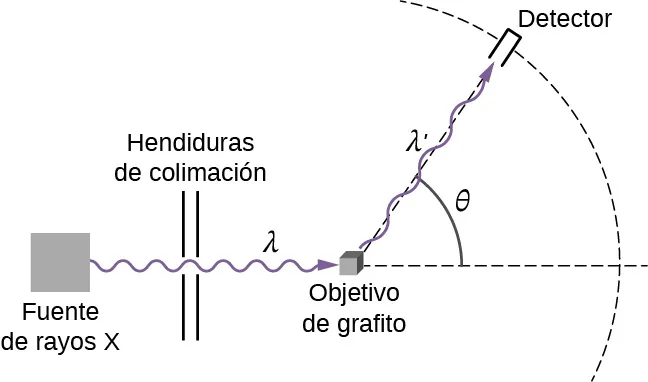
\includegraphics[width=.3\textwidth]{Images/Imagen_2.png}
      \end{center}
\end{wrapfigure}

El efecto Compton es el término utilizado para un resultado
inusual observado cuando los rayos X se dispersan en
algunos materiales. Según la teoría clásica, cuando una
onda electromagnética se dispersa de los átomos, se espera
que la longitud de onda de la radiación dispersada sea la
misma que la de la radiación incidente. En contra de esta
predicción de la física clásica, las observaciones muestran
que cuando los rayos X se dispersan en algunos materiales,
como el grafito, los rayos X dispersados tienen longitudes
de onda diferentes de las de los rayos X incidentes. Este
fenómeno clásicamente inexplicable fue estudiado
experimentalmente por Arthur H. Compton y sus
colaboradores, y Compton dio su explicación en 1923.

Para explicar el desplazamiento de las longitudes de onda
medido en el experimento, Compton utilizó la idea de
Einstein de la luz como partícula. El efecto Compton ocupa
un lugar muy importante en la historia de la física porque
demuestra que la radiación electromagnética no puede
explicarse como un fenómeno puramente ondulatorio. La
explicación del efecto Compton proporcionó un argumento
convincente a la comunidad física de que las ondas
electromagnéticas pueden comportarse en efecto como una
corriente de fotones, lo que situó el concepto de fotón en
una base sólida.

\begin{figure}[H]
      \begin{center}
            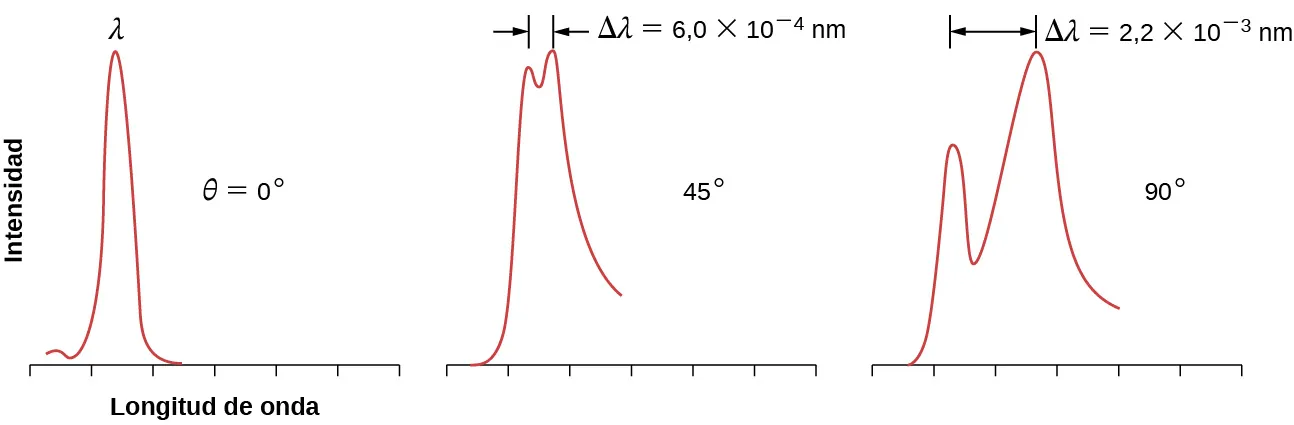
\includegraphics[width=.7\linewidth]{Images/Imagen_3.png}
            \caption{}
      \end{center}
\end{figure}

% + --------------------------------------------------------------|>
\subsection{}

% + --------------------------------------------------------------|>
\subsection{\cite{Moebs_2021}}

El factor $\frac{h}{m_{0} c}$ se llama longitud de onda de
Compton del electrón:

\begin{equation}
      \lambda_{c} = \frac{h}{m_{0} c} = 0.00243 nm = 2.43 pm
\end{equation}

Denotando el desplazamiento como $\Delta \lambda = \lambda'
      - \lambda$, el resultado final puede describirse como:

\begin{equation}
      \Delta \lambda = \lambda_{c} (1 - \cos\theta)
\end{equation}

% + --------------------------------------------------------------|>
\subsection{\cite{Tomé_2019}}

\begin{wrapfigure}{l}{.4\textwidth}
      \begin{center}
            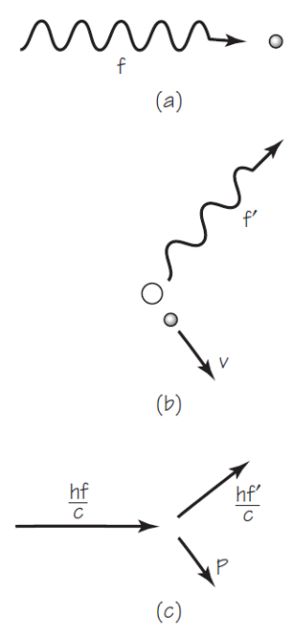
\includegraphics[width=.3\textwidth]{Images/Imagen_4.png}
      \end{center}
\end{wrapfigure}

Arthur Compton calculó cuánta energía debería perder un
fotón en una colisión con un átomo si el momento del fotón
fuese $\frac{h}{\lambda}$. Llegó a la conclusión de que el
cambio en la energía es demasiado pequeño como para poder
observar el efecto mecánico de un fotón en algo tan grande
comparativamente como un átomo completo. Pero si un fotón
golpeara un electrón, que tiene una masa significativamente
más pequeña, el fotón debería transferir una cantidad
significativa de energía al electrón.

En 1923, Compton pudo demostrar que los rayos X se
comportan de hecho como corpúsculos con momento lineal $p =
      \frac{h}{\lambda}$ cuando chocan con electrones. Compton
midió la longitud de onda (o la frecuencia) de los rayos X
incidentes y una vez dispersados y, de esta manera, pudo
determinar el cambio en el momento lineal del fotón de
rayos X. Al medir por separado el momento lineal del
electrón tras la dispersión, pudo verificar que $p =
      \frac{h}{\lambda}$ utilizando la ley de conservación del
momento.

% ! ----------------------------------------------------------------------|>
\section{Resumen del procedimiento}

El experimento implica el uso de un contador de centelleo
calibrado en energía para medir la distribución energética
de los fotones gamma dispersados a diferentes ángulos. Se
realiza una calibración en energía del contador y se
registran los espectros con y sin un material dispersante
de aluminio. A partir de estos datos, se calcula la energía
promedio de los fotones y se verifica la ecuación de
Compton para la dispersión de la radiación gamma. Además,
se calcula la longitud de onda de Compton para el electrón
y se compara con el valor teórico.

\printbibliography

\end{document}